% !TEX root = cha-approach.tex
\documentclass[../../main.tex]{subfiles}

\begin{document}

\section{Initialization}

After extracting the classes and their relationships from the source code, an empty grid is created. The grid is always a square, and its initial size is computed based on the number of classes. The size is intentionally kept small to make the visualization more compact and to help WFC in finding a solution in a computationally efficient manner.

Each cell starts with 15 possible tiles: one empty tile and 14 path tiles. Therefore, each cell is initially in a \emph{superposition} state. The available tiles are shown in \figref{fig:initial_possible_tiles}. They cover the main path shapes, such as straight segments, turns, T-junctions, and crossings. The black segment represents the path, while the gray segment, when present, represents a different path. Each path is identified by a unique ID.

\begin{figure}[ht]
    \centering
    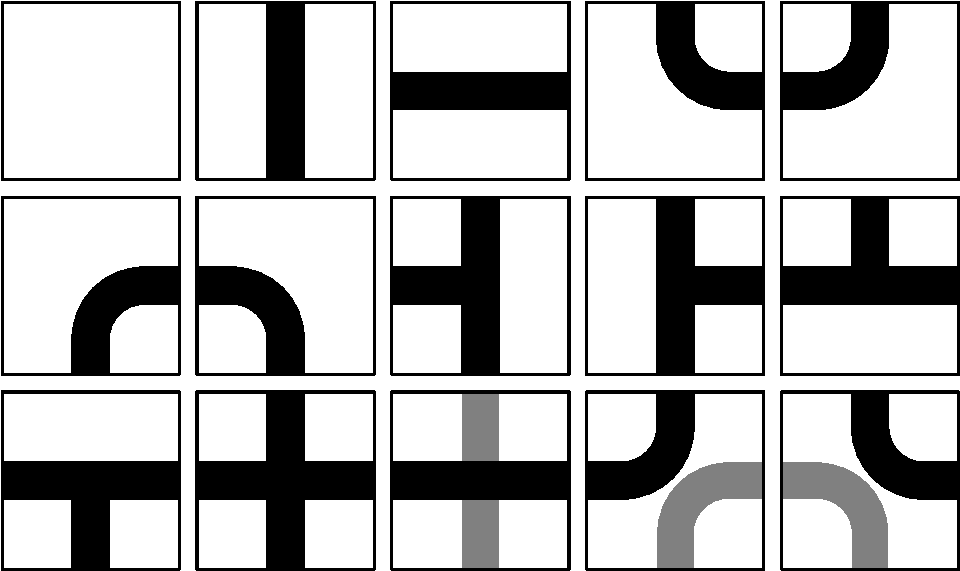
\includegraphics[width=0.5\linewidth]{figures/approach/initial_possible_tiles.pdf}
    \caption{Initial possible tiles.}
    \label{fig:initial_possible_tiles}
\end{figure}

The tiles also define the local constraints used by WFC. These constraints determine which tiles can be placed next to each other. For each tile, the set of compatible tiles is defined separately for each direction (up, left, right and down). An example is shown in \figref{fig:adjancency_rule}, where the straight tile can only be placed next to tiles with matching path segments in each direction.

\begin{figure}[ht]
    \centering
    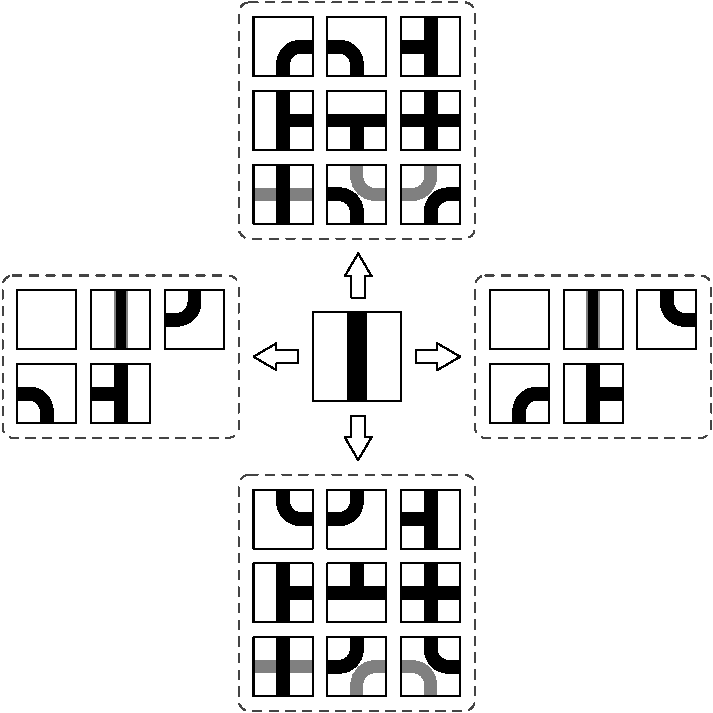
\includegraphics[width=0.85\linewidth]{figures/approach/adjancency_rule.pdf}
    \caption{Example of adjacency constraints for a tile. Compatible tiles are shown for each direction.}
    \label{fig:adjancency_rule}
\end{figure}

Some path tiles cannot be placed on the border of the grid, as they would allow a path to ``leave'' the grid. For example, a vertical path cannot be placed at position $(1,1)$. These invalid tiles are manually removed from the possible tiles of border cells before WFC starts. 
\SL{Dovrei avere aggiungere un'immagine per spiegarla meglio o eliminare direttamente la frase?}